\documentclass[letterpaper]{article}

%\usepackage{fullpage}
%\usepackage{nopageno}
\usepackage{amsmath}
\usepackage{amssymb}
\usepackage{tikz}
\allowdisplaybreaks

\newcommand{\abs}[1]{\left\lvert #1 \right\rvert}

\begin{document}
\title{Notes}
\date{January 16, 2015}
\maketitle
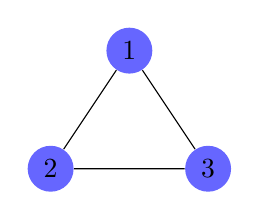
\begin{tikzpicture}[main_node/.style={circle,fill=blue!60,minimum size=1em,inner sep=3pt]}]
    \node[main_node] (1) at (0,0) {1};
    \node[main_node] (2) at (-1, -1.5)  {2};
    \node[main_node] (3) at (1, -1.5) {3};
    \draw (1) -- (2) -- (3) -- (1);
\end{tikzpicture}
\section*{error fixup}
neighborhood is $N_G(V_i)=\{V_j|(v_i,v_j)\in E(G)\}$
\section*{degree sequences}
these will be ascending, book is descending

\subsubsection*{definitionn}
if $G$ is finite with $V(G)=\{v_1,\dots,v_n\}$ such that $d_i=\deg(v_i)\le \deg(v_j)$ for $i\le j$ then $(d_1,\dots,d_n)$ is the degree sequence of $G$.

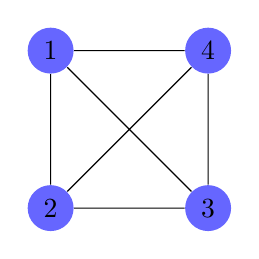
\begin{tikzpicture}[main_node/.style={circle,fill=blue!60,minimum size=1em,inner sep=3pt]}]
    \node[main_node] (1) at (-1,1) {1};
    \node[main_node] (2) at (-1, -1)  {2};
    \node[main_node] (3) at (1, -1) {3};
    \node[main_node] (4) at (1, 1) {4};
    \draw (1) -- (2) -- (3) -- (4) -- (1) -- (3) -- (2) -- (4);
\end{tikzpicture}$=k_4$

$d=(3,3,3,3)$
three regular graph

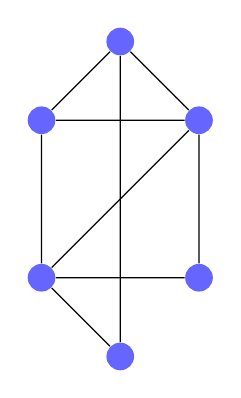
\begin{tikzpicture}[main_node/.style={circle,fill=blue!60,minimum size=1em,inner sep=3pt]}]
    \node[main_node] (1) at (-1,1) {};
    \node[main_node] (2) at (-1, -1)  {};
    \node[main_node] (3) at (1, -1) {};
    \node[main_node] (4) at (1, 1) {};
    \node[main_node] (5) at (0, 2) {};
    \node[main_node] (6) at (0, -2) {};
    \draw (1) -- (2) -- (3) -- (4) -- (1) -- (2) -- (4) -- (5) -- (1);
    \draw (5) -- (6) -- (2) ;
\end{tikzpicture}

$d=(2,3,3,3,3,4)$

\section*{Havel, Hakimi thm}
if $(d_1,\dots,d_n)$ is a non decreasing sequence with $d_n\ge 1$ (avoid the empty graph) it is a degree sequence iff $(d_1,\dots,d_{n-d_n-1},d_{n-d_n}-1,\dots,d_{n-1}-1)$ is a degree sequence
\subsubsection*{example}
given 

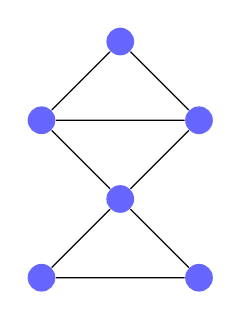
\begin{tikzpicture}[main_node/.style={circle,fill=blue!60,minimum size=1em,inner sep=3pt]}]
    \node[main_node] (1) at (-1,1) {};
    \node[main_node] (2) at (-1, -1)  {};
    \node[main_node] (3) at (1, -1) {};
    \node[main_node] (4) at (1, 1) {};
    \node[main_node] (5) at (0, 0) {};
    \node[main_node] (6) at (0, 2) {};

    \draw (1) -- (4) -- (5) -- (2) -- (3) -- (5) -- (1) -- (6) -- (4);
\end{tikzpicture}

$\to(2,2,2,3,3,4)\to(2,1,1,2,2)$

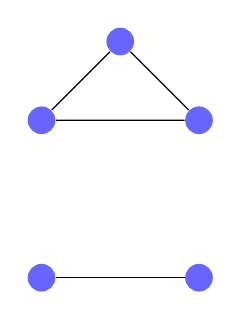
\begin{tikzpicture}[main_node/.style={circle,fill=blue!60,minimum size=1em,inner sep=3pt]}]
    \node[main_node] (1) at (-1,1) {};
    \node[main_node] (2) at (-1, -1)  {};
    \node[main_node] (3) at (1, -1) {};
    \node[main_node] (4) at (1, 1) {};
    %\node[main_node] (5) at (0, 0) {};
    \node[main_node] (6) at (0, 2) {};

    \draw (2) -- (3);
    \draw (1) -- (6) -- (4) -- (1);
\end{tikzpicture}

$(1,1,2,2,2)$

\subsection*{proof}

$\Rightarrow$ careful vertex deletion

$\Leftarrow$ let G have a degree sequeence $*$ then $\deg(v_i)=\begin{cases}d_i&i=1,\dots,n-d_n-1\\d_i-1&i=n-d_n,\dots,n-1\end{cases}$

add a vertex to $G$ and add edges between the new vertex and all vertices of degree $d_i-1$

the degree of the new vertex is $n-1-(n-d_n)+1=d_n$

the new graph has degree sequence $(d_1,\dots,d_n)\Box$

\subsection*{claim}
havel-hakimi can be used to verify, refute the degree sequenceness of any nondecreasing sequence of integers

i.e. we can say rather quickly that (polynomial time) if $(2,3,3,5,5,5,5,5,5,6)$ is graphical 

$n=10, 10-6-1=3, d_3=3, n-d_n=4,d_4-1=4,d_9-1=5$
$(2,3,3,4,4,4,4,4,4)\dots\to\dots (1,1,2,2,2,2)$

question, if two degree sequences are the same, are the graphs isomorphic? no!

\subsection*{homework 1.2}
6a,b,7,10,15
\end{document}
